\documentclass[onecolumn, draftclsnofoot,10pt, compsoc]{article}
\usepackage{graphicx}
\usepackage{url}
\usepackage{lscape}
\usepackage{setspace}
\usepackage{parskip}
\usepackage{geometry}
\usepackage{listings}
\geometry{textheight=9.5in, textwidth=7in}

% 1. Fill in these details
\def \CapstoneTeamName{AgBizClimate}
\def \CapstoneTeamNumber{26}
\def \GroupMemberOne{	Thomas Noelcke}
\def \GroupMemberTwo{	Shane Barrantes}
\def \GroupMemberThree{	Shengpei Yuan}
\def \CapstoneProjectName{ Linking Seasonal Weather Data to AgBizClimate\texttrademark}
\def \CapstoneSponsorCompany{ Oregon State University}
\def \CapstoneSponsorPerson{ Clark Seavert}

% 2. Uncomment the appropriate line below so that the document type works
\def \DocType{		%Software Requirements Document
				%Requirements Document
				%Technology Review
				%Design Document
				Mid Term Progress Report Spring 2018
				}

\newcommand{\NameSigPair}[1]{\par
\makebox[2.75in][r]{#1} \hfil 	\makebox[3.25in]{\makebox[2.25in]{\hrulefill} \hfill		\makebox[.75in]{\hrulefill}}
\par\vspace{-12pt} \textit{\tiny\noindent
\makebox[2.75in]{} \hfil		\makebox[3.25in]{\makebox[2.25in][r]{Signature} \hfill	\makebox[.75in][r]{Date}}}}
% 3. If the document is not to be signed, uncomment the RENEWcommand below
\renewcommand{\NameSigPair}[1]{#1}

%%%%%%%%%%%%%%%%%%%%%%%%%%%%%%%%%%%%%%%
\begin{document}
\begin{titlepage}
    \pagenumbering{gobble}
    \begin{singlespace}
        \hfill
        % 4. If you have a logo, use this includegraphics command to put it on the coversheet.
        %\includegraphics[height=4cm]{CompanyLogo}
        \par\vspace{.2in}
        \centering
        \scshape{
            \huge CS Capstone \DocType \par
            {\large\today}\par
            \vspace{.5in}
            \textbf{\Huge\CapstoneProjectName}\par
            \vfill
            {\large Prepared for}\par
            \Huge \CapstoneSponsorCompany\par
            \vspace{5pt}
            {\Large\NameSigPair{\CapstoneSponsorPerson}\par}
            {\large Prepared by }\par
            Group\CapstoneTeamNumber\par
            % 5. comment out the line below this one if you do not wish to name your team
            %\CapstoneTeamName\par
            \vspace{5pt}
            {\Large
                \NameSigPair{\GroupMemberOne}\par
                \NameSigPair{\GroupMemberTwo}\par
                \NameSigPair{\GroupMemberThree}\par
            }
            \vspace{20pt}
        }
        \begin{abstract}
					 The purpose of this document is to give a snap shot of the current state of the project. In this progress report will start off by discussing ToDo's we have resolved. We will then move on to items that are in progress. After that we will discuss what is still left to do on the project. Next we will give a week by week summary of our progress including our plans for each week, what we accomplished, problems we encountered and a summery for the week. Finally, We will share any new or interesting development, or code from our most recent development cycle.\\
        \end{abstract}
    \end{singlespace}
\end{titlepage}
\newpage
\pagenumbering{arabic}
\tableofcontents
% 7. uncomment this (if applicable). Consider adding a page break.
%\listoffigures 
\newpage
%\listoftables
\clearpage

% 8. now you write!
%this section can likely be coppied from the design doc.
\section{Introduction}
	\subsection{Purpose}
		The purpose of this document is to describe the progress we have made so far on the \textit{AgBizClimate} project. In this document we will give a brief introduction to the \textit{AgBizCliamte} project. In this section we will discuss the purpose of the project. Additionally, we will also discuss the scope of the project and an overview of the project functions.\\
		This document is designed for the project owners. This document is also designed for the development team so we can evaluate our progress so far on this project. This project is also designed to fulfill the minimum requirements for the CS461 class for the OSU computer science program.\\

				\subsection{Overview}
			Seasonal climate is one of the essential factors that affects agricultural production. As a module of \textit{AgBiz Logic}, \textit{AgBizClimate} delivers essential information about climate change to farmers, and help professionals to develop management pathways that best fit their operations under a changing climate. This project aims to link the crucial seasonal climate data from the Northwest Climate Toolbox database to \textit{AgBiz Logic} so that it can provide changes in net returns of crop and livestock enterprises through powerful graphics and tables.\\

		\subsection{Scope}
			This project is a part of a much larger AgBiz Logic\texttrademark program. However, the purpose of this project is to add a short term climate tool to the \textit{AgBizClimate} module. This limits the scope of the project to the \textit{AgBizClimate} Module. Additionally, we will only be adding the short term climate data tool as the long term climate data tool already exists.\\

			Currently \textit{AgBizClimate} has a long-term climate tool but no such tool exists for short term climate data. We will implement a tool to extract short-term climate data from the Northwest Climate Toolbox database, display it to the user and allow the user to adjust crop and livestock yields or quality of products sold and, production inputs. Moreover, a landing tool will be developed to allow users to switch between short-term seasonal tool and long-term climate data tool.\\

		\subsection{Definitions, Acronyms and Abbreviations}
			REST - Representational State Transfer, This is a type of architecture that manages the state of the program. This is especially popular in web development.\\
			API- Application Programming Interface. This is a piece of software that allows a connection to another piece of software providing some sort of service.\\
			NWCTB - Northwest Climate Toolbox. This is the database we will be connecting to that will provide the short term climate data we plan to use.\\
			Thredds Data Server - This is a web server that provides meta-data and data access for scientific data sets using OPeNDAP along with some other remote data access protocols.\\
			OPeNDAP - Open-source Project for a Network Data Access Protocol. This is the protocol we will be using to retrieve the data sets from the Thredds data server.\\
			NMME - North American Multi-Model Ensemble. This is a data set that brings together a variety of different weather models into one data set.\\
			Climate Scenario - This is a theoretical calculation of yields, inputs and of the overall budget for one situation based on the climate data.\\
			NETCDF - This is a file storage format for large scientific data sets especially good for any data that is referenced on a grid and related to is geo-location.\\


		%will need updates.
		\subsection{Product Function Overview}
		    \textit{AgBizClimate} is a web based decision tool that will allow users to gain specific insight on how localized climate data for the next seven months will affect their crop and livestock yields or quality of products sold and production inputs. The \textit{AgBizClimate} tool will allow users to input their location (state, county) and a budget for the specific crop or livestock enterprise. \textit{AgBizClimate} will select climate data for the next seven months for that location and provide graphical data showing temperature and precipitation. Users will then be able to change yields or quality of product sold by a percentage they think these factors will affect and modify production inputs. Finally the tool will calculate the net returns.\\



		\renewcommand\refname{\vskip -1cm}
		\subsection{References}

		    \nocite{*}
            \bibliographystyle{IEEEtran}
            \bibliography{IEEEabrv,References}


\section{Current Project State}
    In this section of this document we will review what items we have resolved, List and explain what items we still have to do, discuss major blockers and give a week by week summary of what we have done so far. This section is intended to give a good overall picture of the status of the \textit{AgBizClimate} project along with what we have accomplished so far.\\

	\subsection{Resolved Items}
		\subsubsection{Create Data Access Tool In R} We created a concept script to try and connect to the database using R rather than python. The goal was to see if could connect to the database and get the data in R rather than python. The goal was to see if the error we were having was in the python library, however, we found we had the same issue as the python code.\\
		
		\subsubsection{Update Expo Poster} We updated the expo poster in prep for expo. We updated the poster to conform with the OSU branding standards and submitted it for printing.\\
		
		\subsubsection{Produce Proof of Concept for Rocket Mount Bind} We wrote some example rocket container to prove that we can use a bind mount to pass and update data to our application in our container. 
		
		\subsubsection{Rewrite API to use local file provided through a mount bind} We updated the API so that it uses the static data provided through the mount bind. We also added to the entry point script to set an environment variable to specify the location of this file.\\
		
		\subsubsection{Write Script for Chron Job} We wrote a script that downloads and updates the data in the file that we want the mount bind to mount. This script will be called by a chron job at the same time every month.\\

	\subsection{In progress}
		\subsubsection{refine API so it fails gracefully} Currently the API will throw exceptions if the file with the climate data does not exist or if the data you are requesting is out of bounds. We are working to make sure that this is handled in a way that returns a useful error to the user that the short term data is unavailable.\\
		
		%Unit testing maybe?
		\subsubsection{Unit Testing} We are in the process of refining the last of the front end tests along with writing unit test to test the updated API.\\
		
		
	\subsection{ToDo's}
		
		\subsubsection{Manual Testing} We need to provide some manual testing to ensure that our addition does not have any bugs. Additionally, we will also need to do some manual testing to ensure that we are not introducing new bugs into the system.\\
		
		\subsubsection{Bug Fixes} Inevitably we will find some bugs through our unit tests and manual testing. We will need to verify and fix bugs found during the testing process.\\
		
		\subsubsection{Document Updates}
			\begin{itemize}
				\item \textbf{Requirements Document} - Update requirements to reflect most recent changes to the project over the last development cycle.
				\item \textbf{Design Document} - Update design document to reflect design as build.
				\item \textbf{Tech Review} - Update tech review to reflect the technology we actually chose to use.
			\end{itemize}

	\subsection{Blockers}
	    In this section we will discuss hurtles we are facing that are impeding progress on this project. We will discuss why they will keep us from moving forward on this project and we will also discuss what we intend to do to move past these problems.\\
			
			\subsubsection{Threadds Server Issues} Through out this project we were required to connect to a threadds server managed at Idaho State University. We've found that all of the various implementations of the NETCDF4 library have the same underlying c library. This c library doesn't work over the network on clunked files. This means that either the Library wasn't made to be used over the network or that there is a serious by in regards to chunked files. This has significantly impeded our progress this term as we've created several implementations of our API with this library to see if we could find a version that would work over the network.\\
			
			\subsubsection{Rocket Issues} We had a really hard time getting rocket set up. The rocket documentation is rather sparse and not always accurate. This really slowed us down on proving that a mount bind would work and would behave how we through in rocket. We were able to overcome this by asking for help from some one who had experience using rocket container.\\


\section{Weekly summary of progress}
	   In this section we will give a weekly summary of our progress on this project. For each we will list out our plans, problems we have encountered during the week and will show a summery of what we have accomplished during the week.\\
		
		\subsection{Week 1}
			\subsubsection{Plans}
			    \begin{itemize}
			        \item Create plan for the term to guarantee we complete project.\\
			        \item Set up some issues in github for project documentation.\\
			        \item Set meeting time with TA.\\
			        \item Set up meeting with Sean.\\
			    \end{itemize}
			\subsubsection{Progress}
			    \begin{itemize}
			        \item Set issues in github.\\
			        \item Tried to set meeting time with TA and emailed multiple times but never got a response.\\
			        \item Set up meeting time for this term with Sean.\\
			    \end{itemize}
			    
			\subsubsection{Problems}
			    \begin{itemize}
			        \item Everyone was sick this week so we were unable to meet as a group.\\
			        \item TA did not respond to our inquiry to set up meeting time for this term.\\
			    \end{itemize}
			\subsubsection{Summary} This week our team decided to take it easy as we we don't expect the work load this term to be to heavy and every one was sick. We did set up some future meetings with our client and tried to set up a meeting with our TA. We also set up some issues in github and started doing some planning to ensure that we are making progress every week.\\
			
		\subsection{Week 2}
			\subsubsection{Plans}
			    \begin{itemize}
			        \item Start working on some unit tests along with some manual testing.\\
			        \item Start working on finishing some of the last development items.\\
			        \item Start adhoc testing.\\
			    \end{itemize}
			\subsubsection{Progress}
			    \begin{itemize}
			        \item Stared working on front end tests. I found an bug in the API that causes it to hang on some requests.\\
			        \item Started working on diagnosis for issue with script.\\
			        \item Started researching alliterative solutions for getting data.\\
			    \end{itemize}
			\subsubsection{Problems}
			    \begin{itemize}
			        \item API isn't returning any data and is hanging forever. I'm not sure why this is, I think the URL may have changed or there is some error with getting the data due to the updated data in the threadds server.
			        \item Found that current solution is not stable and we will need to find a different solution.\\
			    \end{itemize}
			\subsubsection{Summary} This week we did some manual testing and discovered that the climate API was broken. We started looking into potential causes to this issue and potential solutions. Essentially if you can the URL that we are using to get the data it will hang most of the time. This means that the problem is likely in the database we are trying to connect with and that we will need to find a new solution for getting the data. We have some ideas using matlab or R but we will want to produce a concept stript to prove that this will not be an isssue in those languages also.\\
			
		\subsection{Week 3}
			\subsubsection{Plans}
			    \begin{itemize}
			        \item Write matlab API of figure out alternate way to retrieve data.\\
			        \item If we solve data issue start writing unit tests for backend code.
			        \item Add hoc testing.\\
			    \end{itemize}
			\subsubsection{Progress}
			    \begin{itemize}
			        \item Started working on data api using matlab. Discovered that matlab was impossible to use for this purpose as we can't run it in a container and that exporting the interpreter is impractical.\\
			        \item I was able to create an API that used R to try and get the data. However, this implementation produced the same error as the python version.\\
			        \item Met with Sean to discuss possible solutions to this problem. This will probably involve setting up a chron job to get the data every month.\\
			    \end{itemize}
			\subsubsection{Problems}
			    \begin{itemize}
			        \item Our API still isn't returning data and is throwing a fault even in R.\\
			        \item There is a bug in the underlying c library that prevents us from using netcdf4 files over the network. We think that netcdf4 is unable to handle chunked files over the network.\\
			    \end{itemize}
			\subsubsection{Summary} This week we started looking for solutions to our climate data related problems. We discovered that matlab was going to be impossible to use for our particular usecase. We also discovered that R has the same problem as the python version of NETCDF4 in that it throws an exception. The final solution is to set up a cron job on the server that downloads the whole data file and parses it into a mongodb database.\\
			
		\subsection{Week 4}
			\subsubsection{Plans}
			    \begin{itemize}
			        \item Meet to work on and discuss solution to data problems.\\
			        \item Create script to download the data and place it in a database.\\
			        \item Setup Django to use named database for short term data.\\
			        \item Test this solution using a container.\\
			    \end{itemize}
			\subsubsection{Progress}
			    \begin{itemize}
			        \item Stated working on creating the script and databse.\\
			        \item Abandoned idea of using a DB all together and decided that a mount bind to share the directory between the container and the native OS was a better solution.\\
			        \item Started working on a proof of concept for a mount bind.
			    \end{itemize}
			
			\subsubsection{Problems}
			    \begin{itemize}
			        \item Having issues getting docker to run our local docker container.\\
			        \item Having difficulty understanding the devops process for this project.\\
			    \end{itemize}
			
			\subsubsection{Summary} This week we entertained the solution of using mongodb to store our climate database. However after some research and thinking about the problem we decided that the best solution was to use a mount bind. This will allow us to share data between the OS and the container with out the use of a database. We also started working on a proof of concept for this idea, however, we had some difficulties because the support for local docker images through rocket is non-existent.\\
			
		\subsection{Week 5}
			\subsubsection{Plans}
			    \begin{itemize}
			        \item Create concept solution showing that we can bind mount on a native os file in the rocket container. 
			        \item Produce API that uses local version of the NETCDF data file.\\
			        \item Unit testing and manual testing.\\
			        \item Update poster and submit poster for printing.\\
			        \item Complete Midterm progress report.\\
			    \end{itemize}
			\subsubsection{Progress}
			    \begin{itemize}
			        \item Produced a proof of concept demonstrating that a bind mound will behave how we expect.\\
			        \item Re-implemented API to use local NETCDF file.\\
			        \item Wrote midterm progress report.\\
			        \item Created midterm progress report presentation and video.\\
			        \item Set up API so it fails gracefully when the data file doesn't exist or the data the user requests isn't in the data file.\\
			    \end{itemize}
			\subsubsection{Problems}
			no problems this week.\\
			\subsubsection{Summary} This week we made a lot of progress on the API. Most of this weeks efforts have been aimed at re-writing the API to use a local file to provide the data. In the production application this data will be provided through a mount bind. Additionally the location of this file is provided through a configuration value in the settings.py file so that it can be specified differently for the production environment. We also set up the API to handle many different errors including invalid input, no data file and data not existing within the daata file.\\
			
% what do we want to put here?
\section{Interesting Code}
In this section we will discuss  a piece of code that is interesting, and essential to our application. Our production application is run in the containerization system known as rkt created by CoreOS. Due to this use of containerization and limited permission access on the production server we are unable to download the entire climate dataset from the Northwest Climate Toolbox directly to the container. Instead, we have created a monthly cron job on the native OS (not in the container) that will download the entire climate data set and store it on the production server. We will then remake the container and apply a bind mount which allows the container and therefore AgBizClimate to access the climate data on the native OS. This will allow us to query the dataset with our original API while bypassing the network NETCDF chunking issues.

  \begin{figure}[!htb]
	  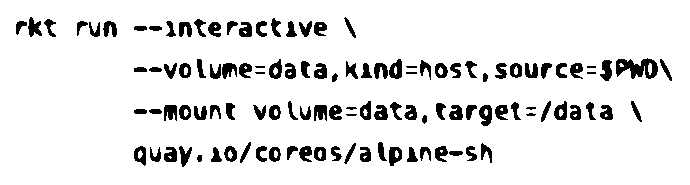
\includegraphics[width=0.8\textwidth,natwidth=610,natheight=642]{interesting_code.eps}
	  \caption{rkt-run.sh - Bind Mount}
  \end{figure}

\end{document}
